\documentclass[12pt,letterpaper]{lsuetdmod}
\usepackage{amsfonts}
\usepackage{anyfontsize}
\usepackage{amsmath,amssymb,amsthm}
\usepackage{bm}
\usepackage{graphicx}
\usepackage{float}
\usepackage{multicol}
\usepackage{multirow}
\usepackage{mathtools}
\usepackage{enumerate}
\usepackage{threeparttable}
\usepackage{tabularx}
\usepackage{siunitx}
\usepackage[export]{adjustbox}
\usepackage[breaklinks=true]{hyperref}
\usepackage{setspace,graphics,dsfont,verbatim,indentfirst}
\usepackage{paralist}
\usepackage{arydshln}
\usepackage[labelsep=period]{caption}
\usepackage{bookmark}
\usepackage[linesnumbered, ruled, vlined]{algorithm2e}
\usepackage{algorithmic}
\usepackage{lipsum}

\setcounter{MaxMatrixCols}{10}

\setlength{\topmargin}{-0.5in}
\setlength{\textheight}{9.0in}
\addtolength{\evensidemargin}{-0.50in}
\addtolength{\oddsidemargin}{-0.50in}
\addtolength{\textwidth}{1.00in}
\setlength{\parindent}{1.75em}
\setlength{\parskip}{0ex}
\setcounter{tocdepth}{1} % Set the depth of table of contents

\hypersetup{pdfborder={0 0 0}} % Set the hyperref box hidden

\newtheorem{thm}{Theorem}
\numberwithin{thm}{chapter}
\newtheorem{lem}{Lemma}
\numberwithin{lem}{chapter}
\newtheorem{cor}{Corollary}
\numberwithin{cor}{chapter}
\newtheorem{prop}{Proposition}
\newtheorem{defn}{Definition}
\numberwithin{defn}{chapter}
\newtheorem{cond}{Condition}
\numberwithin{cond}{chapter}
\newtheorem{rmk}{Remark}
\numberwithin{rmk}{chapter}

\DeclareMathOperator{\atantwo}{atan2}
\DeclareMathOperator{\acos}{acos}
\DeclareMathOperator{\arctantwo}{arctan2}
\DeclareMathOperator{\scgt}{SCgt}

\makeatletter
%\def\@makefnmark{\hbox{\normalfont\@thefnmark} }
% Put dots after headings (e.g. "1.1.2. Sectionname")
\usepackage{secdot}
\sectiondot{chapter}
\sectiondot{section}
\sectiondot{subsection}
\sectiondot{subsubsection}

% Put dots after heading numbers in the ToC (e.g. "1.1.2. Sectionname")
\usepackage[dotinlabels]{titletoc}

% Change appearance of Appendix in ToC  (e.g. "A "becomes "Appendix A")
\usepackage[titletoc]{appendix}

% Put footnote to the bottom of the page
\usepackage[bottom]{footmisc}

% Footer redefine: in text number is superscript style; in footer number is normal size.
\long\def\@makefntext#1{%
	\parindent 1em\noindent \hb@xt@ 1.8em{\hss \normalfont\scriptsize\@thefnmark}\enskip #1}

% 
\newcommand\blfootnote[1]{%
	\begingroup
	\renewcommand\thefootnote{}\footnote{#1}%
	\addtocounter{footnote}{-1}%
	\endgroup
}

\usepackage{array}
\newcolumntype{L}[1]{>{\raggedright\let\newline\\\arraybackslash\hspace{0pt}}m{#1}}
\newcolumntype{C}[1]{>{\centering\let\newline\\\arraybackslash\hspace{0pt}}m{#1}}
\newcolumntype{R}[1]{>{\raggedleft\let\newline\\\arraybackslash\hspace{0pt}}m{#1}}

\usepackage{tablefootnote}
%\usepackage{pdfpages}

\usepackage[defaultlines=2,all]{nowidow}
\setnowidow
\setnoclub


\begin{document}
\renewcommand\@pnumwidth{1.55em}
\renewcommand\@tocrmarg{9.55em}
\renewcommand*\l@chapter{\@dottedtocline{0}{1.5em}{2.3em}}
\renewcommand*\l@figure{\@dottedtocline{1}{0em}{3.1em}}
\let\l@table\l@figure

\pagenumbering{roman}
\thispagestyle{empty}
\begin{center}
%The title page is first created. large -> titlesize: 14pt ->16pt
\newcommand{\titlesize}{\fontsize{16pt}{20pt}\selectfont}
{\bfseries\titlesize DISTANCE-BASED FORMATION CONTROL: THEORY, APPLICATIONS, AND ISSUES}

\vfill
\doublespacing
A Dissertation \\
\singlespacing
Submitted to the Graduate Faculty of the \\
Louisiana State University and \\
Agricultural and Mechanical College \\
in partial fulfillment of the \\
requirements for the degree of \\
Doctor of Philosophy \\
\doublespacing
in \\
                                       
The Department of Mechanical and Industrial Engineering \\
\singlespacing
\vfill

by \\
Tairan Liu \\
B.S., University of Science and Technology of China, 2012  \\
May 2020
\end{center}
\pagebreak
%The Copyright Page and Dedication sections can be added here, if desired.



%\chapter*{Copyright Page}
\thispagestyle{empty}
\begin{center}
	\vspace*{\fill}
	\doublespacing
	Copyright \textcopyright \ 2020 \\
	Tairan Liu \\
	All rights reserved\\
	\vspace*{\fill}
\end{center}

%Insert the appropriate text for the copyright page here.
%\addcontentsline{toc}{chapter}{\hspace{-1.5em} {COPYRIGHT PAGE} \vspace{12pt}}
\pagebreak

%\chapter*{Dedication}
%\doublespacing
%\vspace{0.55ex}
%Insert the appropriate text for the dedication or epigraph page here.  This part of the ETD must not exceed one page.
%\addcontentsline{toc}{chapter}{\hspace{-1.5em} {DEDICATION} \vspace{12pt}}
%\pagebreak

\chapter*{Acknowledgments}
\doublespacing
\vspace{0.55ex}
I would like to $\ldots$.



%The code below adds the Acknowledgments section to the Table of Contents.
\addcontentsline{toc}{chapter}{\hspace{-1.3em}{ACKNOWLEDGMENTS} }
\addtocontents{toc}{\vspace{12pt}}
\pagebreak


%The Preface section can now be added, if desired.

%\chapter*{Preface}
%\doublespacing
%\vspace{0.55ex}
%Insert the appropriate text for the preface here.
%\addcontentsline{toc}{chapter}{\hspace{-1.5em} {PREFACE} \vspace{12pt}}
%\pagebreak

\singlespacing
\pdfbookmark[chapter]{TABLE OF CONTENTS}{toc}
\tableofcontents
\pagebreak
\singlespacing


\renewcommand\@pnumwidth{1.55em}
\renewcommand\@tocrmarg{8.55em}


\cleardoublepage\phantomsection
\addcontentsline{toc}{chapter}{\hspace{-1.5em} LIST OF TABLES}
%\doublespacing
\addtocontents{toc}{\vspace{12pt}}
\listoftables
\pagebreak
\singlespacing


\cleardoublepage\phantomsection
\addcontentsline{toc}{chapter}{\hspace{-1.5em} LIST OF FIGURES}
\addtocontents{toc}{\vspace{12pt}}
\listoffigures
\pagebreak



%The List of Nomenclature may be included here, if desired.

%\chapter*{List of Nomenclature}
%\doublespacing
%\vspace{0.55ex}
%Provide the definitions of the symbols used in your thesis or dissertation here.
%\addcontentsline{toc}{chapter}{\hspace{-1.5em} LIST OF NOMENCLATURE \vspace{12pt}}
%\pagebreak

%The code below adds the Abstract and places it within the Table of Contents.
\cleardoublepage\phantomsection
\renewenvironment{abstract}{{\hspace{-2.2em} \Large \textbf{\abstractname}} \par}{\pagebreak} %huge
\addcontentsline{toc}{chapter}{\hspace{-1.5em} ABSTRACT}
\addtocontents{toc}{\vspace{12pt}}


\begin{abstract}
\vspace{0.55ex}
\doublespacing
This research $\ldots$.


\end{abstract}

\pagenumbering{arabic}
\addtocontents{toc}{\hspace{-1.4em}{CHAPTER} \vspace{-1em}}
\singlespacing
\setlength{\textfloatsep}{12pt plus 2pt minus 2pt}
\setlength{\intextsep}{6pt plus 2pt minus 2pt}


\chapter{Introduction} \label{ch:intro}
\doublespacing
\section{Motivation}

\lipsum[1-5]

\section{Literature Review}

\subsection{XXX}

Based on ... \cite{khalil2015nonlinear}:
\begin{compactenum}[1.]
	\item something;
	
	\item something;
	
	\item something.
\end{compactenum}

\nocite{*}
\lipsum[6-7]

\subsection{YYY}

\lipsum[8-9]

\begin{figure}[htbp]
	\centering
	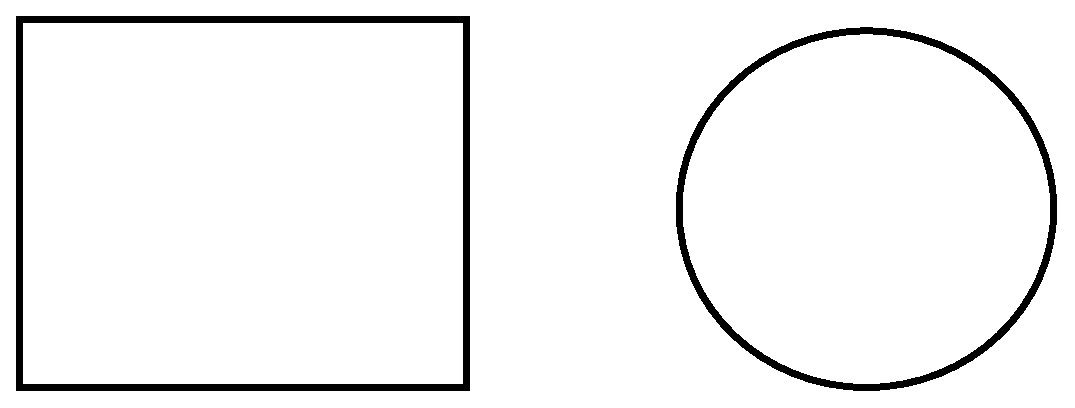
\includegraphics[width=0.7\linewidth]{Pics/intro/drawing}
	\caption{This is a very short caption.}
	\label{fig:drawing}
\end{figure}

\begin{figure}[htbp]
	\centering
	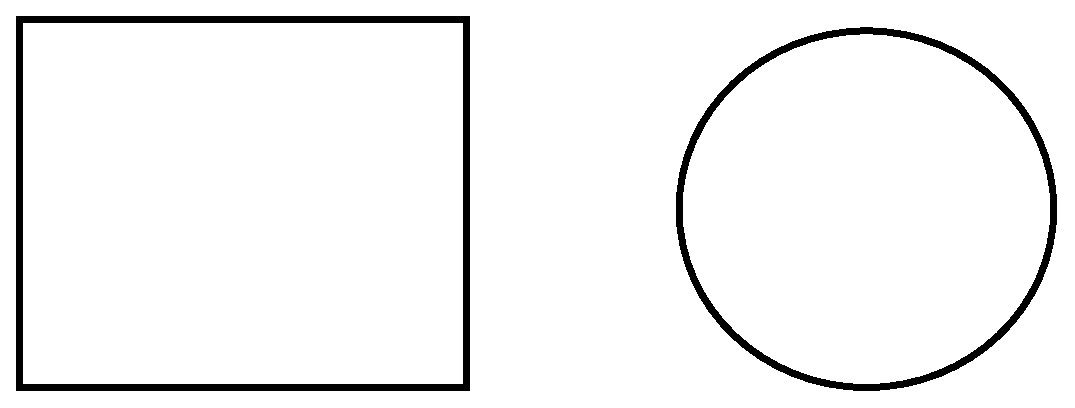
\includegraphics[width=0.7\linewidth]{Pics/intro/drawing}
	\caption{This is a very short caption.}
	\label{fig:drawing2}
\end{figure}

\begin{figure}[htbp]
	\centering
	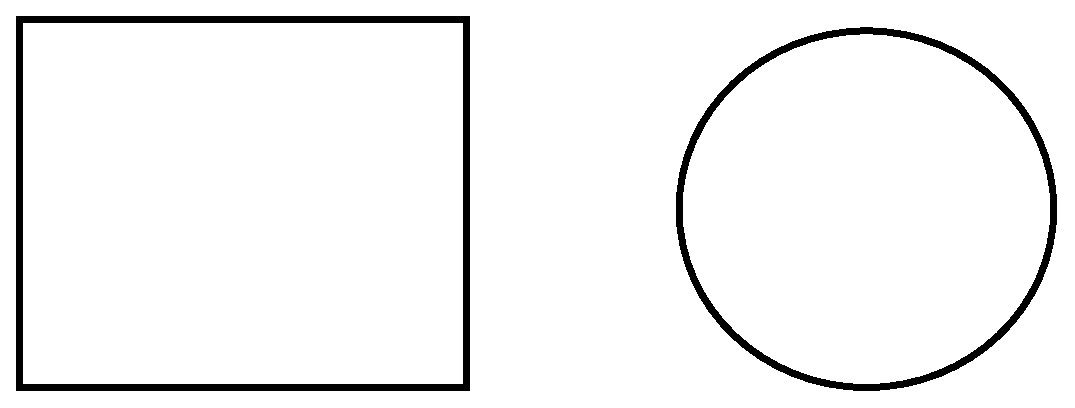
\includegraphics[width=0.7\linewidth]{Pics/intro/drawing}
	\caption{This is a very short caption.}
	\label{fig:drawing3}
\end{figure}

\lipsum[10-11]
Two examples are given in Figure \ref{fig:drawing}: .... Figure \ref{fig:drawing2} .... Figure \ref{fig:drawing3}.


\section{Dissertation Organization}

This dissertation ....

\begin{table}[hbp]
	\caption[Major topics in each chapter.]{Major topics in each chapter.}
	\label{tab:topic-in-chapter}
	\centering
	\begin{tabular}{l | c | c | c | c | c}
		\hline
		\quad & Xx & Xx & Xx & Xx\tablefootnote{Xxx.} & Xx \\
		\hline
		Chapter xx & \checkmark & & \checkmark & \checkmark &  \\
		\hline
		Chapter xx & \checkmark & & \checkmark & &  \\
		\hline
		Chapter xx & \checkmark & & \checkmark & & \checkmark \\
		\hline
		Chapter xx & & \checkmark & \checkmark & &  \\
		\hline
		Chapter xx & \checkmark & \checkmark & \checkmark & & \\
		\hline
		Chapter xx & \checkmark & \checkmark & & \checkmark & \checkmark\\
		\hline
	\end{tabular}
\end{table}

\lipsum[12-14]



\pagebreak
\singlespacing


\chapter{Notation and Basic Concepts} \label{ch:notation-concepts}
\doublespacing
\lipsum[20-23]

\begin{table}[hbp]
	\caption[XXX.]{XXX.}
	\label{tab:topic-in-chapter}
	\centering
	\begin{tabular}{l | c | c | c | c | c}
		\hline
		\quad & xx & xx & xx & xx\tablefootnote{Xxx.} & xx \\
		\hline
		Xx & \checkmark & & \checkmark & \checkmark &  \\
		\hline
		Xx & \checkmark & & \checkmark & &  \\
		\hline
		Xx & \checkmark & & \checkmark & & \checkmark \\
		\hline
		Xx & & \checkmark & \checkmark & &  \\
		\hline
		Xx & \checkmark & \checkmark & \checkmark & & \\
		\hline
		Xx & \checkmark & \checkmark & & \checkmark & \checkmark\\
		\hline
	\end{tabular}
\end{table}

\lipsum[24-26]

\begin{table}[hbp]
	\caption[XXX.]{XXX.}
	\label{tab:topic-in-chapter}
	\centering
	\begin{tabular}{l | c | c | c | c | c}
		\hline
		\quad & xx & xx & xx & xx\tablefootnote{Xxx.} & xx \\
		\hline
		Xx & \checkmark & & \checkmark & \checkmark &  \\
		\hline
		Xx & \checkmark & & \checkmark & &  \\
		\hline
		Xx & \checkmark & & \checkmark & & \checkmark \\
		\hline
		Xx & & \checkmark & \checkmark & &  \\
		\hline
		Xx & \checkmark & \checkmark & \checkmark & & \\
		\hline
		Xx & \checkmark & \checkmark & & \checkmark & \checkmark\\
		\hline
	\end{tabular}
\end{table}

\lipsum[27-28]





\pagebreak
\singlespacing


\chapter{System Models} \label{ch:system-model}
\doublespacing
%\input{SystemModels}
\pagebreak
\singlespacing



\chapter{Summary} \label{ch:sum-future}
\doublespacing
%\input{SummaryFutureWork}
\pagebreak
\singlespacing


\addtocontents{toc}{\vspace{12pt}}
\addtocontents{toc}{\hspace{-1.8em} {APPENDIX} \vspace{-1em}}
\appendix

\chapter{Additional Proofs}
\doublespacing
%\input{AdditionalProofs}
\pagebreak
\singlespacing


\chapter{Additional Calculation}
\doublespacing
%\input{DetailedCalculation}
\pagebreak
\singlespacing


\chapter{Letter of Copyright Permission}
\vspace{0.5em}
%\input{CopyrightPermission}
\pagebreak





\addtocontents{toc}{\vspace{12pt}}
\addcontentsline{toc}{chapter}{\hspace{-1.5em} REFERENCES}
\renewcommand{\bibname}{References\vspace{0.5em}}
%\begin{thebibliography}{999}
%\vspace{0.9em}
%\input{Bibliography}
%\end{thebibliography}
\bibliographystyle{IEEEtr}
\bibliography{References}
% When changes are made to references, use bibliograpy to generate the mainfile.bbl file, then copy the content inside in to the Bibliograph file, and enable thebibliography environment.
\pagebreak
\singlespacing


%Finally, the vita section is created and included in the Table of Contents.
\chapter*{Vita}
\doublespacing
\setlength{\parindent}{1.75em}
\vspace{0.2em}
\addtocontents{toc}{\vspace{12pt}}
\addcontentsline{toc}{chapter}{\hspace{-1.5em} VITA}
%\input{Vita}
%Insert the text of your vita, which is basically a description of yourself and your academic career.




\end{document}





